
\chapter{MOOC: Kalman Filter}


\section{Least-Squares}
\subsection{Quadratic function}
A quadratic function has the following form:
\begin{equation}
    f(x) = \underbrace{x^T Q x}_{quadratic} + \underbrace{L x + c}_{affine}
\end{equation}


$Q$ could have different values. To have a unique notation, we enforce $Q$ to be symmetric.

\subsubsection{Jacobian of quadratic function}
Identifying it in Taylor development:

\begin{equation}
\begin{split}
    f(x + \delta x) &= (x+\delta x)^T Q (x + \delta x) \\
    &= x^T Q x + x^T Q \delta x + \delta x^T Q x + \delta x^T Q \delta x \\
    &= \underbrace{x^T Q x}_{f(x)} + \underbrace{2 x^T Q}_{J_f}  \delta x + o(||\delta x||)
\end{split}
\end{equation}

Thus, the Jacobian the quadratic part is:
\begin{equation}
    \frac{\delta f}{\delta x}(x) = 2 x^T Q
\end{equation}

If the function has an affine part non null, the full Jacobian of is:
\begin{equation}
    \frac{\delta f}{\delta x}(x) = 2 x^T Q + L
\end{equation}



\subsubsection{Eigen values}
As $Q$ is symmetric, we have:
\begin{itemize}
    \item eigen values are real
    \item eigen vectors are orthogonal
\end{itemize}

If eigen values of $Q$ are striclty positive, $Q$ is said positive definite.

\begin{itemize}
    \item $\lambda_1 > 0, \lambda_2 > 0 \longrightarrow$  paraboloid
    \item $\lambda_1 > 0, \lambda_2 < 0 \longrightarrow$  saddle point
    \item $\lambda_1 < 0, \lambda_2 < 0 \longrightarrow$  reversed paraboloid
\end{itemize}


\begin{figure}[H]
    \centering
    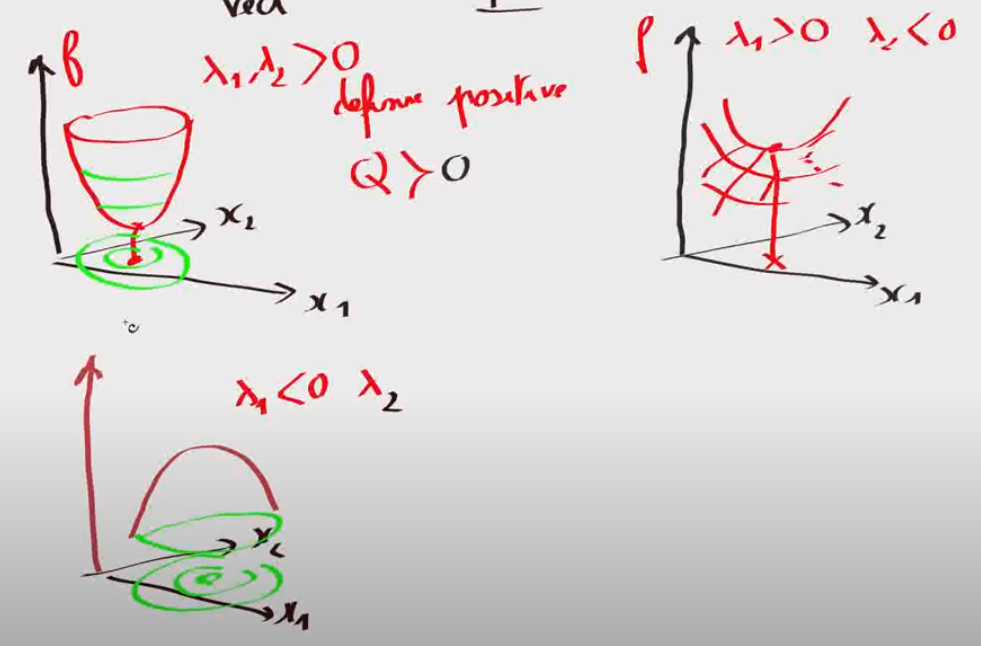
\includegraphics[scale=0.3]{content/Quadratic_function_eigen_values.png}
    \caption{Form of quadrics dependeing to eigen values signs.}
    \label{fig:resnet}
\end{figure}

\subsection{Least-squares}

To solve $f(p) = y$, where $f$ is a linear function $f(p) = M p$, we define a criteria:
\begin{equation}
    c(p) = ||f(p)-y||^2 = ||M p-y||^2
\end{equation}
We want to minimize this criteria. The term "least-squares" comes from the square.

\begin{equation}
\begin{split}
    c(p) &= ||M p-y||^2  \\
    &= (Mp-y)^T(Mp-y) \\
    &=p^T M^T M p - 2 y^T M p + y^t y \\
    &=p^T \underbrace{M^T M}_{Q} p \underbrace{- 2 y^T M}_{L}p + \underbrace{y^t y}_{c} \\
\end{split}
\end{equation}

We get a quadratic function, so we can minimize it by finding where the derivative is null ($\frac{\delta f}{\delta p}(\hat{p}) = 0$).
\begin{equation}
\begin{split}
2 \hat{p}^T M^TM -2y^T M &= 0 \\
\hat{p}^T M^TM &= y^TM \\
M^T M \hat{p} &= M^T y \\
\hat{p} &= (M^T M)^{-1} M^T y \\
\end{split}
\end{equation}

This matrix $(M^T M)^{-1} M^T = K$ is called an \textbf{estimator}.
$\hat{y} = M \hat{p} = M K y$ is called the filtered measures.



\textbf{WARNING !!!} $(M^TM)$ needs to be invertible, and thus, $M$ needs to have full rank.

\section{Parameters estimation}
\subsection{Minmization}

In the general case, we try to minimize a function $f$, $f: \mathbb{R}^n \longrightarrow \mathbb{R}$.
\begin{figure}[H]
    \centering
    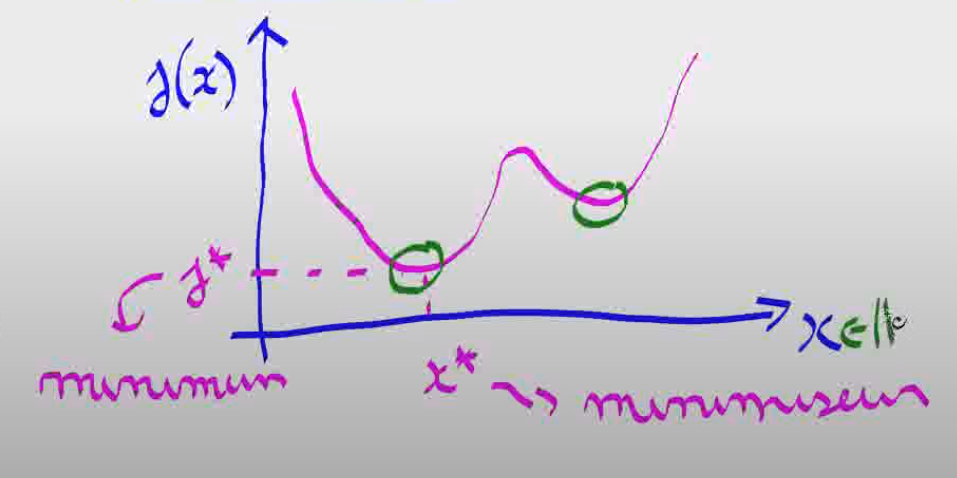
\includegraphics[scale=0.3]{content/minimization.png}
    \caption{Minimize a general function can have local minima.}
    \label{fig:minmization}
\end{figure}

In the class of problems that try to minimize a quadratic criteria, the function has the following shape:

\begin{figure}[H]
    \centering
    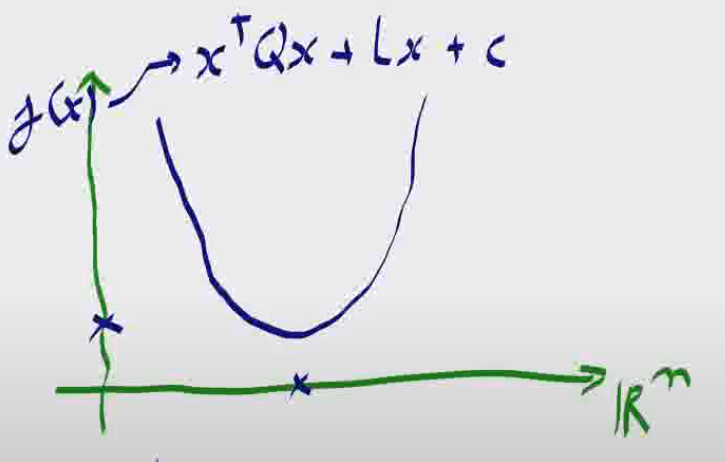
\includegraphics[scale=0.3]{content/minimization_quadratic.png}
    \caption{Quadratic criteria}
    \label{fig:minimization_quadratic}
\end{figure}

The function has the following form: $J(x) = x^T Q x + Lx + c$ and we find the minimum by zeroing the derivative.

\begin{equation}
    \frac{\delta j}{\delta x} = 2 x^T Q + L = 0
\end{equation}

and thus the minimum $x*$ has the following expression:

\begin{equation}
    x* = -\frac{1}{2}Q^{-1}L^T
\end{equation}




\subsection{Parameters estimation}

\begin{figure}[H]
    \centering
    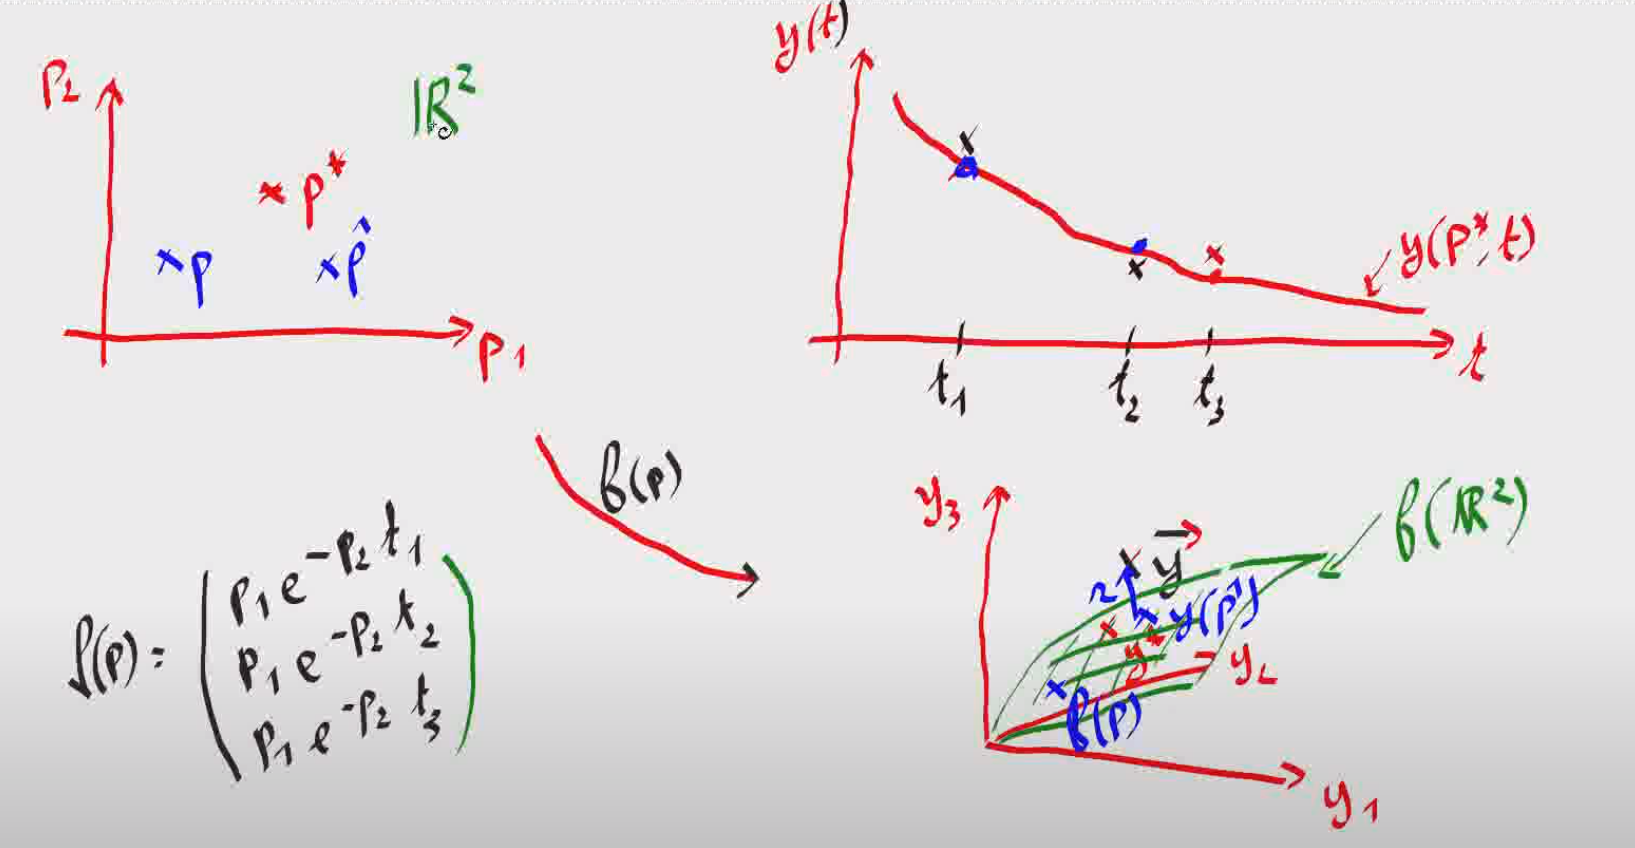
\includegraphics[width=\linewidth]{content/params_estimation.png}
    \caption{Parameters estimation}
    \label{fig:params_estimation}
\end{figure}

The "best" estimate of the parameters in the sense of the least-squares is the projection of the measure $y$ on the surface formed by the image of all the possible values for the parameters $p_1, p_2$.



In case of a linear model ($Mp$), the image of the parameters is a plane. $y$ is the measure, $\hat{y}$ is the filtered measure and has an antecedent $\hat{p}$ which is the estimated parameters. It can be computed with the pseudo-inverse.

\begin{figure}[H]
    \centering
    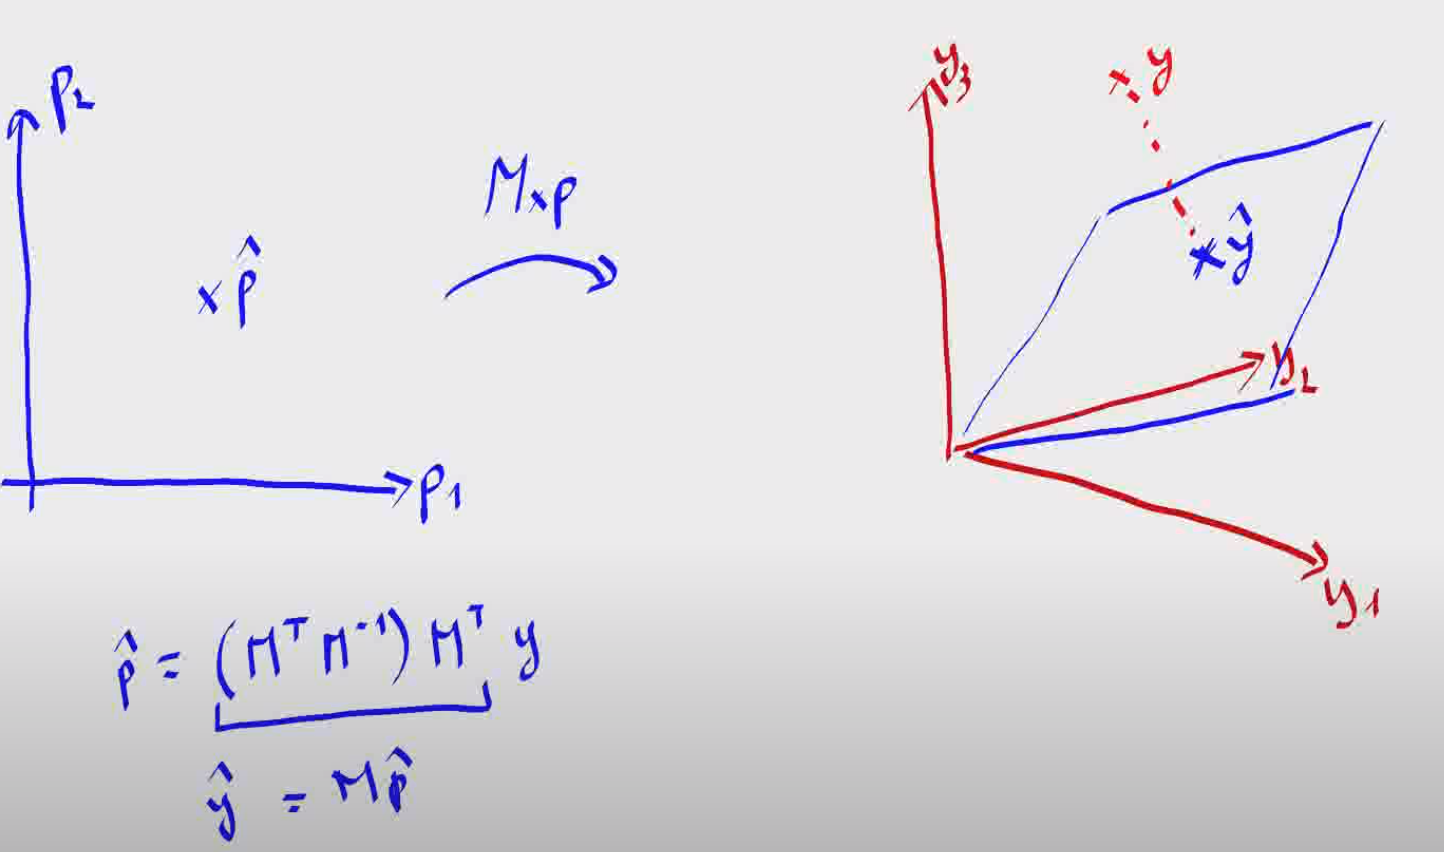
\includegraphics[width=\linewidth]{content/estimation_linear_model.png}
    \caption{Parameters estimation in a linear model}
    \label{fig:params_estimation_linear_model}
\end{figure}

We can also consider the function $\mathbb{R}^2 \longrightarrow \mathbb{R}$ which associates the norm of the vector $\overrightarrow{Mpy}$ to a parameter $p$. In case of a linear model, this function is quadratic and can be minimized.

\begin{figure}[H]
    \centering
    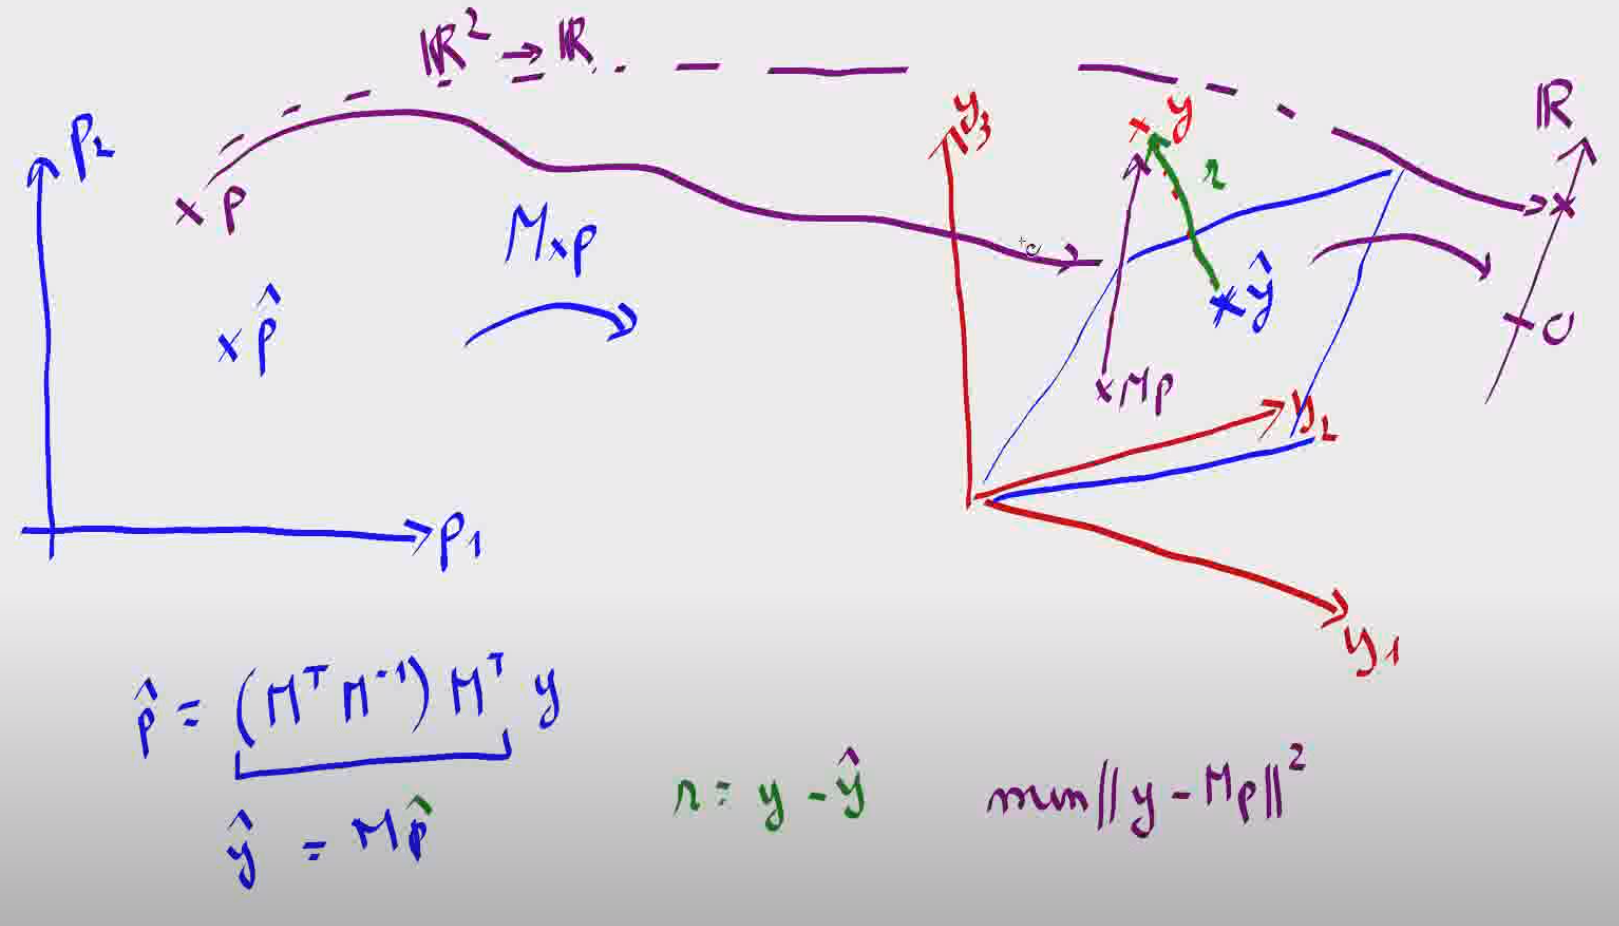
\includegraphics[width=\linewidth]{content/estimation_linear_model_2.png}
    \caption{Parameters estimation in a linear model}
    \label{fig:params_estimation_linear_model_2}
\end{figure}



\subsection{Newton's Method}

In the least-squares approach, we want to minimize $||f(p)-y||^2$. 
\begin{itemize}
    \item if $f$ is linear, there is an analytical solution in closed form.
    \item if $f$ is non-linear, we need to linearize it iteratively.
\end{itemize}


\subsubsection{Linearization}
In case where $f$ is non-linear in $j(p) = ||f(p)-y||^2$, we linearize it at the current point.

\begin{equation}
\begin{split}
    j(p) &= \norm{f(p_0) + \frac{\delta f}{\delta p}(p_0) (p-p_0)}^2 \\
    &= \norm{\underbrace{\frac{\delta f}{\delta p}(p_0)}_{M} p + \underbrace{f(p_0) - \frac{\delta f}{\delta p}(p_0)p_0 - y}_{-z}}^2 \\
    j(p) &= \norm{Mp - z}^2
\end{split}
\end{equation}

This time, it is linear and we have the analytical solution:
\begin{equation}
    p_1 = (M^TM)^{-1}M^Tz = p_0 + (M^TM)^{-1}M^T (y-f(p_0))
\end{equation}
This is then repeated for $p_2$, $p_3$, ...
 
\begin{algorithm}[H]
\DontPrintSemicolon
\KwInput{$p_0$: starting point}
\KwOutput{}
For $k=0$ to $k_{max}$\\
$M = \frac{\delta f}{\delta p}(p_k)$ \\
$p_{k+1}= p_k + (M^TM)^{-1}M^T (y-f(p_k))$
\caption{Newton's algorithm}
\end{algorithm}

\begin{figure}[H]
    \centering
    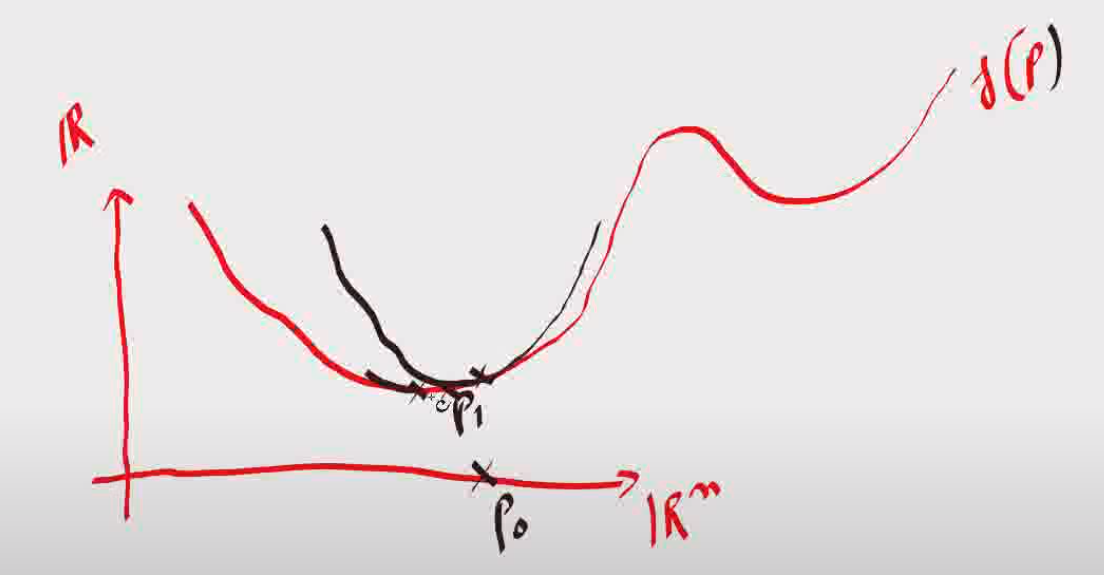
\includegraphics[width=\linewidth]{content/newton_algorithm.png}
    \caption{Through linearization of $f$, the residual function $j(p)$ is approximated with a parabole (quadratic function) in Newton's method}
    \label{fig:params_estimation_linear_model_2}
\end{figure}

\subsection{Monte-Carlo Method}

Also known as \textbf{Simulated annealing} (recuit simule). This method can be used to avoid local minimum.


\begin{algorithm}[H]
\DontPrintSemicolon
\KwInput{$p$: starting point}
\KwOutput{}
$T = 1$ \\
Choose random $d \in \mathbb{R}^n $\\
$q = p + d * T$ \\
\uIf{$j(q) < j(p)$}{
$p=q$
}
$T = 0.99 \times T$ \\
Repeat
\caption{Monte-Carlo's method}
\end{algorithm}

$T$ is called the "temperature" and controls the size of the steps: large at the beginning, smaller after.



\section{Covariance Matrices}

A simple covariance matrix has the form:
\begin{equation}
    G = \left(\begin{array}{cc}
        \sigma_1^2 & 0 \\
        0 & \sigma_2^2
    \end{array}\right)
\end{equation}

This corresponds to the first 2x2 block of the dual form matrix of the ellipse with axes $\sigma_1, \sigma_2$.
The primal form of this ellipse is:
\begin{equation}
    A = \left(\begin{array}{cc}
        1/\sigma_1^2 & 0 \\
        0 & 1/\sigma_2^2
    \end{array}\right)
\end{equation}

and the corresponding equation is $\frac{x^2}{\sigma_1^2}+\frac{y^2}{\sigma_2^2} = 1$. When we consider just the ellipse, its axes are the standard deviation of the corresponding distribution (with the corresponding covariance matrix).
Using the $\chi^2$ law, we can draw the confidence ellipse of a covariance matrix at a certain degree of probability.
To do that, the axes, so $\sigma_1$ and $\sigma_2$ are scaled by $\sqrt{-2\ln{(1-p)}}$, where $p$ is the probability that the ellipse contains a sample.


For example, drawing the ellipse with $\sigma_1$ and $\sigma_2$ as axes corresponds to a scale factor of 1, and thus we have $\sqrt{-2\ln{(1-p)}} = 1$.
This corresponds to a probability:
\begin{equation}
    p = 1-\exp^{-\frac{1}{2}} = 0.3935
\end{equation}


All of this can also be applied to rotated and non-centered ellipses. In that case, the covariance matrix corresponds to the 2x2 block of the \textbf{re-centered} dual form matrix.


\newpage
\begin{equation}
    \sigma_1
\end{equation}
\begin{equation}
    \color{cyan}  \sigma_2
\end{equation}
\begin{equation}
    \sigma_3
\end{equation}
\begin{equation}
    \sigma_4
\end{equation}
\begin{equation}
    \sigma_5
\end{equation}
\begin{equation}
    \theta
\end{equation}

\begin{equation}
    \color{green}  \Delta \theta_2
\end{equation}


\begin{equation}
\begin{split}
    \theta\\
    a\\
    b\\
    (c_x, c_y)
    \end{split}
\end{equation}


\begin{equation}
    \begin{split}
         P = K[Rt] \\
        C^* = P Q^* P^T
    \end{split}
\end{equation}

(with $P = K[Rt]$)

\begin{equation}
    \begin{split}
         &a, b \\
         &\theta \\
         &c_x, c_y
    \end{split}
\end{equation}


\begin{equation}
    \mathcal{L}_{bin} = -\log \left(\frac{\exp(bin_{gt})}{\sum_j \exp(bin_j)}\right)
\end{equation}